การออกแบบ labeling tool นั้น ผู้วิจัยได้เลือกใช้แพลตฟอร์ม PyQt และภาษา Python ในการพัฒนา
เนื่องจากแพลติฟอร์ม PyQt นั้นเป็นแพลตฟอร์มที่มีผู้พัฒนาใช้กันอย่างแพร่หลาย จึงทำให้สะดวกในการศึกษาและหาข้อมูลผ่านอินเตอร์เน็ต
อีกทั้งยังเป็นแพลตฟอร์มที่สามารถพัฒนาด้วยภาษา Python ได้ และเป็นแพลตฟอร์มที่ใช้งานง่าย สามารถปรับปรุงแก้ไขได้ง่าย
เนื่องจากการสร้างแอพพลิเคชั่นนั้นจำเป็นต้องมีการปรับแก้หน้าต่างอยู่เสมอ

\subsection{แอพพลิเคชั่น labeling tool}
ภาพรวมของแอพพลิเคชั่นที่สร้างขึ้นประกอบด้วยส่วน Select, Detect, Track และ Action label
เพื่อช่วยแบ่งเบาภาระของผู้พัฒนาในการสร้าง label สำหรับสร้างโมเดลจากข้อมูลประเภทวิดีโอ โดยส่วน Select
จะต้องสามารถตัดวิดีโอส่วนที่ไม่มีมนุษย์อยู่ออกจากวิดีโอได้ Detect ต้องสามารถหาตำแหน่งของมนุษย์ภายในวิดีโอได้
Track ต้องสามารถทำนายตำแหน่งต่อไปของมนุษย์ข้อมูลตำแหน่งของมนุษย์จาก Detect ได้
Action label ต้องสามารถทำนายการกระทำของมนุษย์ได้ในระดับหนึ่ง โดยทุกส่วนการทำงานมนุษย์ต้องสามารถทำงานร่วมกับระบบได้
ดังรูปที่ \ref{fig:labeling_overview}

\begin{figure}[!ht]
    \centering
    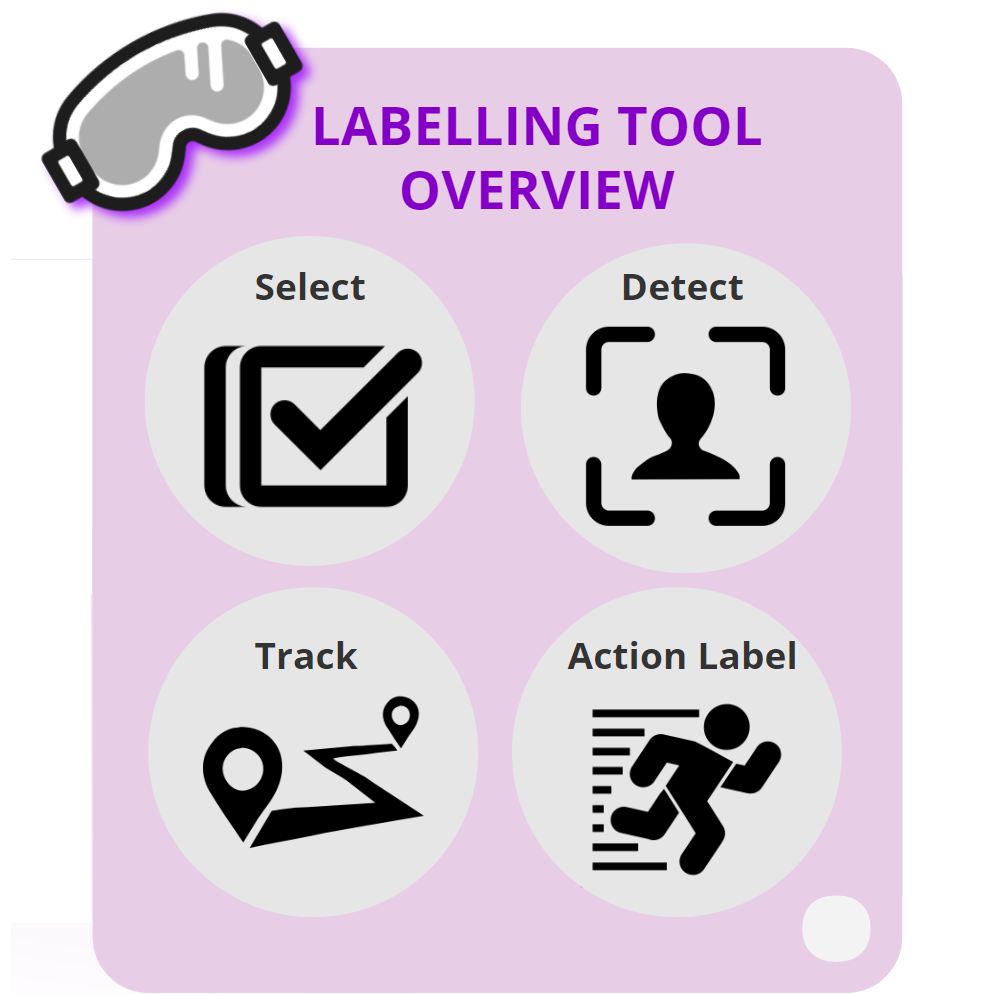
\includegraphics[width=0.7\textwidth]{chapter3/images/3_3/labelingToolOverview.png}
    \caption{ภาพรวมระบบของแอพพลิเคชั่น labeling tool}
    \label{fig:labeling_overview}
\end{figure}

\clearpage
\subsection*{โดยแต่ละส่วนจะมีรายละเอียดดังนี้}
\subsubsection{Select}
ในส่วนของแถบ Select จะมีหน้าต่างเป็นดังรูปที่ \ref{fig:selectTab} โดยในส่วนนี้จะมีหน้าที่ในการโหลดวิดีโอที่ต้องการ
กำหนดอัตราการหยิบตัวอย่างเฟรมของวิดีโอแล้วเก็บเฟรมเหล่านั้นเป็นคีย์เฟรม(Keyframe) และตัดวิดีโอส่วนที่ไม่มีมนุษย์อยู่ออกไป
\begin{figure}[!ht]
    \centering
    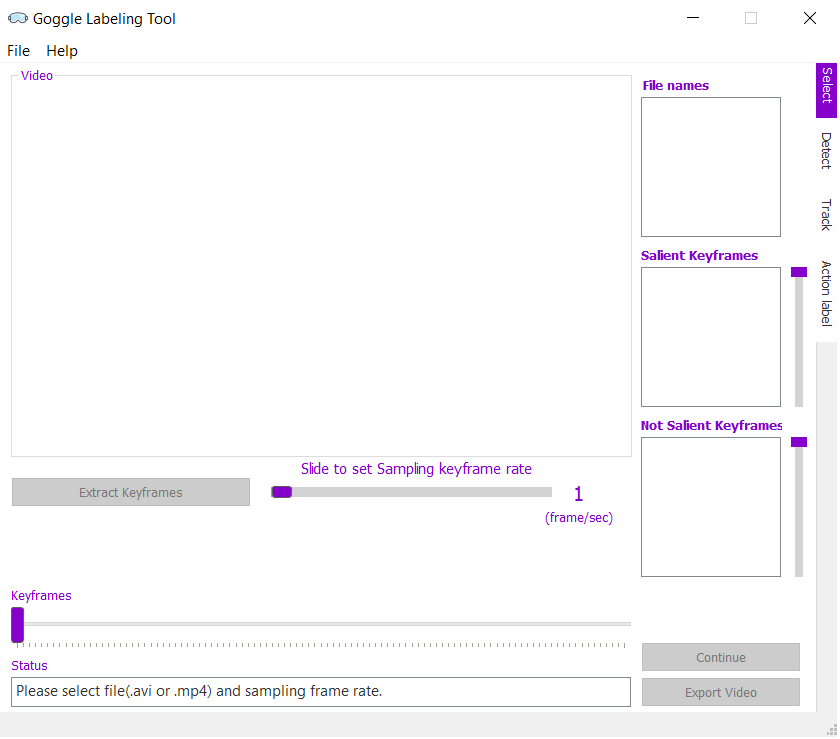
\includegraphics[width=1\textwidth]{chapter3/images/3_3/SelectTab.png}
    \caption{หน้าต่างแถบ Select ของแอพพลิเคชั่น labeling tool}
    \label{fig:selectTab}
\end{figure}
\clearpage
ซึ่งในขั้นตอนการตัดส่วนวิดีโอที่ไม่มีมนุษย์อยู่นั้น ได้ใช้โมเดล YoLo-v3 320 สำหรับตรวจหามนุษย์ในแต่ละคีย์เฟรม
จากนั้นจะแยกคีย์เฟรมที่มีมนุษย์อยู่ และที่ไม่มีมนุษย์อยู่ออกมา แล้วเก็บไว้ในช่องรายการหมายเลข 1 และ 2 ตามลำดับ
ดังรูปที่ \ref{fig:SelectTab_sampled}

\begin{figure}[!ht]
    \centering
    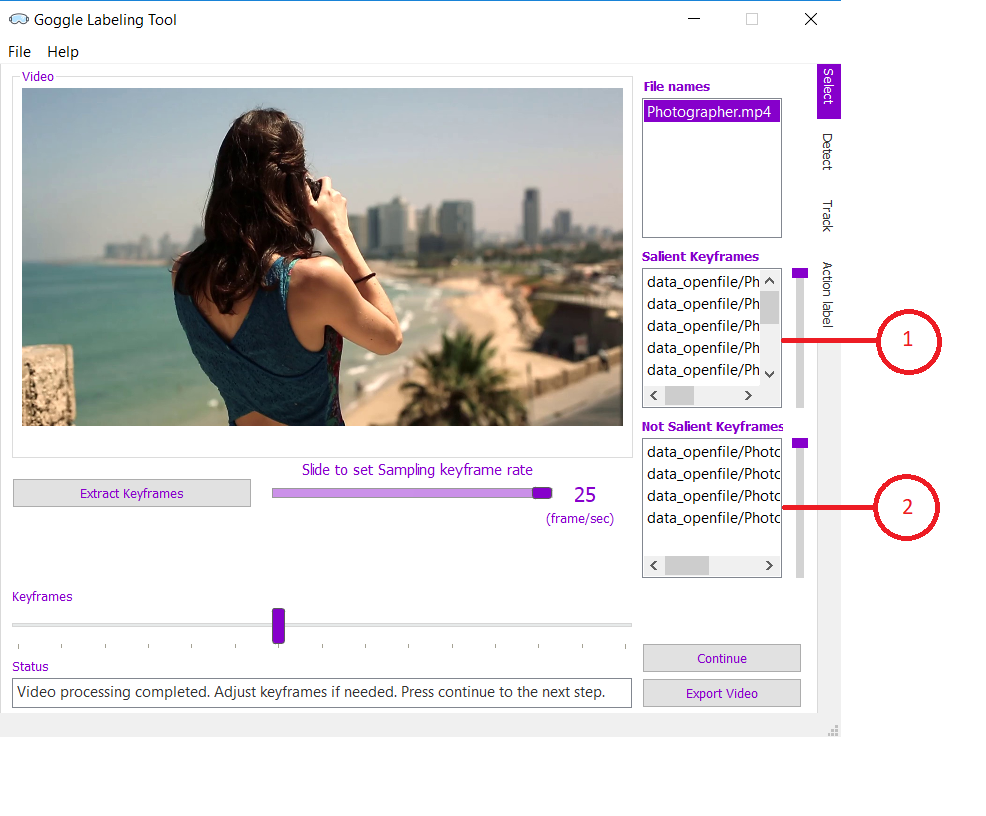
\includegraphics[width=1\textwidth]{chapter3/images/3_3/SelectTab_sampled.png}
    \caption{หลังจากตัดส่วนวิดีโอแล้ว คีย์เฟรมจะถูกเก็บไว้ในช่องรายการตามประเภท}
    \label{fig:SelectTab_sampled}
\end{figure}
\clearpage
\subsubsection{Detect}
ในส่วนของแถบ Delect จะมีหน้าต่างเป็นดังรูปที่ \ref{} โดยในส่วนนี้จะมีหน้าที่ในการ

\begin{figure}[!ht]
    \centering
    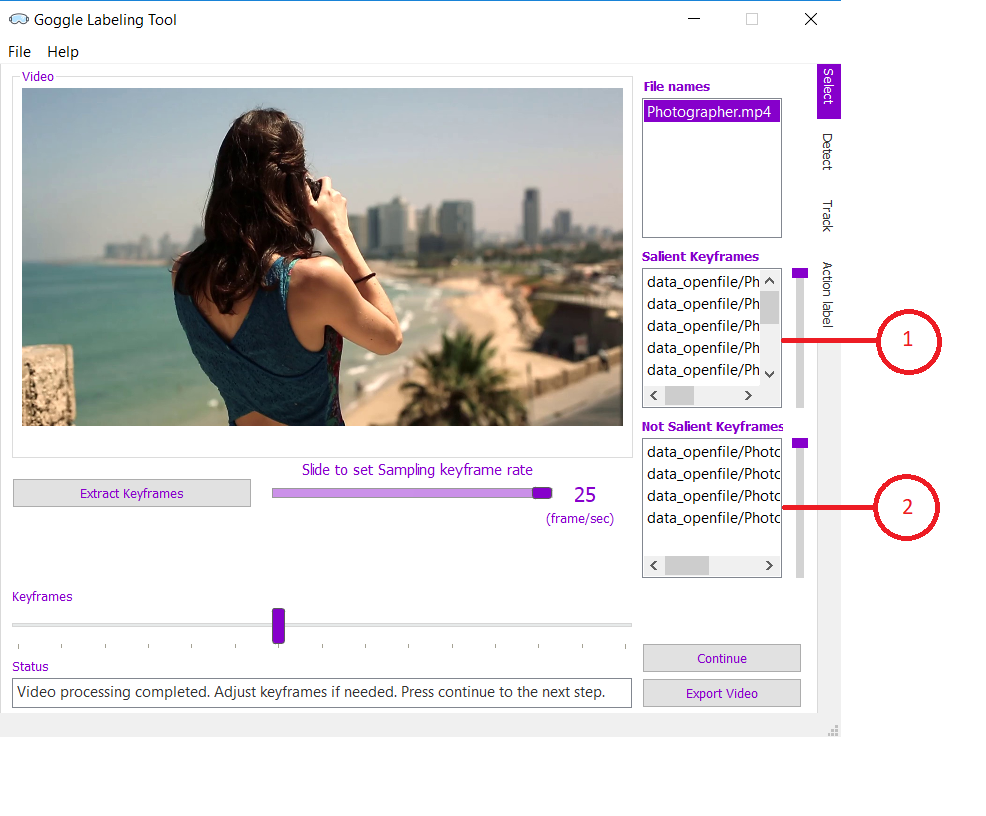
\includegraphics[width=1\textwidth]{chapter3/images/3_3/SelectTab_sampled.png}
    \caption{หลังจากตัดส่วนวิดีโอแล้ว คีย์เฟรมจะถูกเก็บไว้ในช่องรายการตามประเภท}
    \label{fig:SelectTab_sampled}
\end{figure}
% \begin{table}[!ht]
% 	\centering
% 	\begin{tabular}{| l | l | l |}
% 		\hline
% 		Properties & ABS & PLA \\
%         \hline
%         Tensile Strength & 27 $MPa$ & 37 $MPa$ \\
%         Elongation & 3.5 \- 50\% & 6\% \\
%         Flexural Modulus & 2.1 \- 7.6 $GPa$ & 4 $GPa$ \\
%         Density & 1.0 - 1.4 $g/cm^3$ & 1.3 $g/cm^3$ \\
%         Melting Point & 230$°C$ - 240$°C$ & 215$°C$ - 235$°C$ \\ 
%         การย่อยสลายทางธรรมชาติ & ไม่ได้ & ได้ (ภายใต้เงื่อนไขที่ถูกต้อง) \\
% 	    \hline
% 	\end{tabular}
% 	\caption{ตารางแสดงสมบัติทางกลของวัสดุพลาสติก}
% 	\label{tab:plastic_material_properties}
% \end{table}
